\subsubsection{Guest Use Cases}
The Guest actor is restricted to public discovery and account access. The most
important public use cases are account registration, training path
consultation, certificate verification, and search.


\subsubsubsection[Browse Training Content]{Refinement of the Use Case Browse Training Content} Figure
\ref{fig:guest-browse-training-content-use-case} presents the refinement of the
Use Case Browse Training Content for the Guest actor. This use case includes
the following sub-use cases:
\begin{figure}[H]
    \centering
    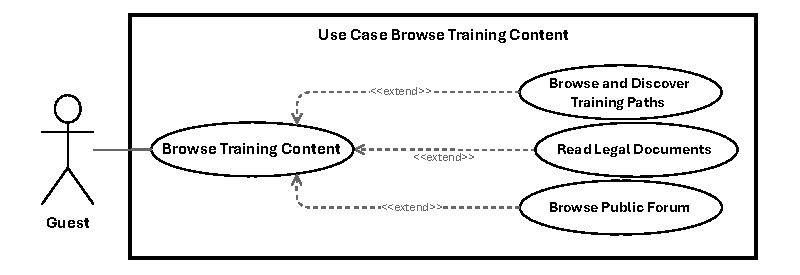
\includegraphics[width=\textwidth]{assets/chapter3/guest-browse-training-content-use-case}
    \caption{Use Case Browse Training Content}
    \label{fig:guest-browse-training-content-use-case}
\end{figure}
\dotsection{\textbf{Specification of the Use Case Browse and Discover Training Paths}}
\begin{table}[H]
    \centering
    \caption{Use Case Specification: Browse and Discover Training Paths}
    \begin{tabular}{|p{3.5cm}|p{10.5cm}|}
        \hline
        \textbf{Title}          & Browse and Discover Training Paths \\
        \hline
        \textbf{Summary}        & Guest discovers available training paths by viewing the landing page, searching and filtering the catalog, and reading detailed path information including syllabus, reviews, pricing, and instructor details \\
        \hline
        \textbf{Actor}          & Unauthenticated User (Guest) \\
        \hline
        \textbf{Precondition}   & The platform is publicly accessible and at least one training path is published \\
        \hline
        \textbf{Post-condition} & Guest has viewed platform offerings and has enough information to decide whether to register \\
        \hline
        \textbf{Basic Scenario} & \begin{minipage}[t]{\linewidth}
            \begin{enumerate}[topsep=0pt,itemsep=1pt,parsep=0pt,partopsep=0pt]
                \item Guest arrives at the platform homepage; system displays featured training paths with titles, descriptions, and ratings
                \item Guest navigates to the catalog; system lists all published training paths with categories, ratings, and pricing
                \item Guest enters a keyword or selects category filters; system returns ranked matching results that may be sorted by price, rating, or enrollment count
                \item Guest selects a training path; system displays the full detail page including description, learning objectives, module syllabus, pricing, duration, instructor profile, and enrolled-engineer statistics
                \item Guest may read course reviews on the detail page to evaluate quality before deciding to register
                \item If the guest attempts to enroll, the system redirects to the registration page
            \end{enumerate}
        \end{minipage} \\
        \hline
        \textbf{Error Scenario} & \begin{minipage}[t]{\linewidth}
            \begin{enumerate}[topsep=0pt,itemsep=1pt,parsep=0pt,partopsep=0pt]
                \item If no featured paths are configured, the landing page displays a default welcome message
                \item If no paths match the search criteria, the system displays a no-results message with suggestions
                \item If the search service is unavailable, the system falls back to a static listing with a retry option
                \item If a selected training path is not found or unpublished, the system redirects to the catalog
            \end{enumerate}
        \end{minipage} \\
        \hline
    \end{tabular}
    \label{tab:guest-browse-discover}
\end{table}
\dotsection{\textbf{Specification of the Use Case Read Legal Documents}}
\begin{table}[H]
    \centering
    \caption{Use Case Specification: Read Legal Documents}
    \begin{tabular}{|p{3.5cm}|p{10.5cm}|}
        \hline
        \textbf{Title}          & Read Legal Documents \\
        \hline
        \textbf{Summary}        & Any user reads the platform's Terms of Service or Privacy Policy to understand usage rights and data handling practices \\
        \hline
        \textbf{Actor}          & Unauthenticated User (Guest), Engineer, Teacher, Administrator \\
        \hline
        \textbf{Precondition}   & The requested legal document is available and accessible \\
        \hline
        \textbf{Post-condition} & User views the complete and latest version of the selected legal document \\
        \hline
        \textbf{Basic Scenario} & \begin{minipage}[t]{\linewidth}
            \begin{enumerate}[topsep=0pt,itemsep=1pt,parsep=0pt,partopsep=0pt]
                \item User navigates to the legal section via footer links
                \item User selects either \textbf{Terms of Service} or \textbf{Privacy Policy}
                \item System retrieves the latest version of the selected document
                \item System renders the document in a readable, properly formatted view
                \item User scrolls through and reads the complete document
            \end{enumerate}
        \end{minipage} \\
        \hline
        \textbf{Error Scenario} & \begin{minipage}[t]{\linewidth}
            \begin{enumerate}[topsep=0pt,itemsep=1pt,parsep=0pt,partopsep=0pt]
                \item If the document is unavailable or fails to load, the system displays a friendly error message with a retry option
            \end{enumerate}
        \end{minipage} \\
        \hline
    \end{tabular}
    \label{tab:guest-legal-docs}
\end{table}
\dotsection{\textbf{Specification of the Use Case Browse Public Forum}}
\begin{table}[H]
    \centering
    \caption{Use Case Specification: Browse Public Forum}
    \begin{tabular}{|p{3.5cm}|p{10.5cm}|}
        \hline
        \textbf{Title}          & Browse Public Forum \\
        \hline
        \textbf{Summary}        & Guest browses and reads public forum threads and their replies to follow community discussions without authentication \\
        \hline
        \textbf{Actor}          & Unauthenticated User (Guest) \\
        \hline
        \textbf{Precondition}   & The platform is publicly accessible and the forum contains at least one published thread \\
        \hline
        \textbf{Post-condition} & Guest has read one or more forum threads and their approved replies \\
        \hline
        \textbf{Basic Scenario} & \begin{minipage}[t]{\linewidth}
            \begin{enumerate}[topsep=0pt,itemsep=1pt,parsep=0pt,partopsep=0pt]
                \item Guest navigates to the public forum page; system displays a paginated list of threads with titles, authors, and reply counts
                \item Guest may sort threads by date, popularity, or category, or search by keyword
                \item Guest selects a thread; system displays the full detail page showing the original post with author and timestamp, followed by all approved replies in chronological order
                \item Guest reads the discussion and may view engagement metrics
                \item If the guest attempts to post or reply, the system redirects to the registration page
            \end{enumerate}
        \end{minipage} \\
        \hline
        \textbf{Error Scenario} & \begin{minipage}[t]{\linewidth}
            \begin{enumerate}[topsep=0pt,itemsep=1pt,parsep=0pt,partopsep=0pt]
                \item If no threads match a search query, the system displays a no-results message
                \item If a selected thread is not found or has been removed, the system displays a not-found notice and returns to the listing
            \end{enumerate}
        \end{minipage} \\
        \hline
    \end{tabular}
    \label{tab:guest-browse-forum}
\end{table}

\iffalse
\dotsection{\textbf{Specification of the Use Case View Landing Page}}
\begin{table}[H]
    \centering
    \caption{Use Case Specification: View Landing Page}
    \begin{tabular}{|p{3.5cm}|p{10.5cm}|}
        \hline
        \textbf{Title}          & View Landing Page                                                                               \\ \hline
        \textbf{Summary}        & Guest views the landing page with featured courses preview to discover available training paths \\ \hline
        \textbf{Actor}          & Unauthenticated User (Guest)                                                                    \\ \hline
        \textbf{Precondition}   & The platform is publicly accessible and featured training paths are configured                  \\ \hline
        \textbf{Post-condition} & The guest views the landing page with featured courses and platform overview                    \\ \hline
        \textbf{Basic Scenario} & \begin{minipage}[t]{\linewidth}
                                      \begin{enumerate}[topsep=0pt,itemsep=1pt,parsep=0pt,partopsep=0pt]
                                          \item Guest navigates to the platform homepage
                                          \item System displays the landing page with featured training paths
                                          \item System shows course previews including titles, descriptions, and ratings
                                          \item Guest may browse featured courses and navigate to detailed views
                                      \end{enumerate}
                                  \end{minipage}           \\ \hline
        \textbf{Error Scenario} & \begin{minipage}[t]{\linewidth}
                                      \begin{enumerate}[topsep=0pt,itemsep=1pt,parsep=0pt,partopsep=0pt]
                                          \item If no featured courses are configured, the system displays a default welcome
                                                message
                                          \item If the landing page fails to load, the system shows a friendly error message
                                      \end{enumerate}
                                  \end{minipage}       \\ \hline
    \end{tabular}
    \label{tab:guest-landing-page}
\end{table}
\dotsection{\textbf{Specification of the Use Case Search Training Paths}}
\begin{table}[H]
    \centering
    \caption{Use Case Specification: Search Training Paths}
    \begin{tabular}{|p{3.5cm}|p{10.5cm}|}
        \hline
        \textbf{Title}          & Search Training Paths                                                                                              \\
        \hline
        \textbf{Summary}        & Guest searches and filters public training path listings to discover available learning content before registering \\
        \hline
        \textbf{Actor}          & Guest                                                                                                              \\
        \hline
        \textbf{Precondition}   & The platform is publicly accessible and at least one training path is published                                    \\
        \hline
        \textbf{Post-condition} & The guest views filtered training path results matching their search criteria                                      \\
        \hline
        \textbf{Basic Scenario} & \begin{minipage}[t]{\linewidth}
                                      \begin{enumerate}[topsep=0pt,itemsep=1pt,parsep=0pt,partopsep=0pt]
                                          \item Guest navigates to the training paths catalog page
                                          \item System displays published training paths with titles, categories, ratings, and
                                                pricing
                                          \item Guest enters a search keyword or selects category filters
                                          \item System returns matching training paths ranked by relevance
                                          \item Guest may sort results by price, rating, or enrollment count
                                          \item Guest selects a training path to view its detailed description and syllabus
                                      \end{enumerate}
                                  \end{minipage}                        \\
        \hline
        \textbf{Error Scenario} & \begin{minipage}[t]{\linewidth}
                                      \begin{enumerate}[topsep=0pt,itemsep=1pt,parsep=0pt,partopsep=0pt]
                                          \item If no training paths match the search criteria, the system displays a
                                                no-results message with suggestions
                                          \item If the search service is unavailable, the system shows a fallback listing and
                                                retry option
                                          \item If the guest attempts to enroll, the system redirects to the registration page
                                      \end{enumerate}
                                  \end{minipage}                        \\
        \hline
    \end{tabular}
    \label{tab:guest-search-training-paths}

\end{table}
\dotsection{\textbf{Specification of the Use Case View Training Path Details}}
\begin{table}[H]
    \centering
    \caption{Use Case Specification: View Training Path Details}
    \begin{tabular}{|p{3.5cm}|p{10.5cm}|}
        \hline
        \textbf{Title}          & View Training Path Details                                                                                 \\ \hline
        \textbf{Summary}        & Guest views detailed information about a specific training path including syllabus and learning objectives \\ \hline
        \textbf{Actor}          & Unauthenticated User (Guest)                                                                               \\ \hline
        \textbf{Precondition}   & The training path is published and publicly accessible                                                     \\ \hline
        \textbf{Post-condition} & The guest views comprehensive training path information                                                    \\ \hline
        \textbf{Basic Scenario} & \begin{minipage}[t]{\linewidth}
                                      \begin{enumerate}[topsep=0pt,itemsep=1pt,parsep=0pt,partopsep=0pt]
                                          \item Guest selects a training path from the catalog or search results
                                          \item System displays the training path detail page
                                          \item System shows the training path title, description, and objectives
                                          \item System displays the syllabus with modules and training units
                                          \item System shows pricing, duration, and instructor information
                                          \item Guest may view reviews and enrollment statistics
                                      \end{enumerate}
                                  \end{minipage}                             \\ \hline
        \textbf{Error Scenario} & \begin{minipage}[t]{\linewidth}
                                      \begin{enumerate}[topsep=0pt,itemsep=1pt,parsep=0pt,partopsep=0pt]
                                          \item If the training path is not found, the system displays a not-found message
                                          \item If the training path is unpublished, the system redirects to the catalog
                                      \end{enumerate}
                                  \end{minipage}                    \\ \hline
    \end{tabular}
    \label{tab:guest-view-details}
\end{table}
\dotsection{\textbf{Specification of the Use Case Read Terms of Service}}
\begin{table}[H]
    \centering
    \caption{Use Case Specification: Read Terms of Service}
    \begin{tabular}{|p{3.5cm}|p{10.5cm}|}
        \hline
        \textbf{Title}          & Read Terms of Service                                                                           \\ \hline
        \textbf{Summary}        & Guest views the platform's Terms of Service document to understand usage rights and obligations \\ \hline
        \textbf{Actor}          & Unauthenticated User (Guest), Engineer, Teacher, Administrator                                  \\ \hline
        \textbf{Precondition}   & The Terms of Service document is available and accessible                                       \\ \hline
        \textbf{Post-condition} & The guest views the complete Terms of Service document                                          \\ \hline
        \textbf{Basic Scenario} & \begin{minipage}[t]{\linewidth}
                                      \begin{enumerate}[topsep=0pt,itemsep=1pt,parsep=0pt,partopsep=0pt]
                                          \item Guest navigates to the legal section via footer links
                                          \item Guest selects the Terms of Service option
                                          \item System retrieves the latest version of the Terms of Service
                                          \item System renders the document in a readable format with proper formatting
                                          \item Guest may scroll through and read the complete document
                                      \end{enumerate}
                                  \end{minipage}            \\ \hline
        \textbf{Error Scenario} & \begin{minipage}[t]{\linewidth}
                                      \begin{enumerate}[topsep=0pt,itemsep=1pt,parsep=0pt,partopsep=0pt]
                                          \item If the document is unavailable, the system displays a friendly error message
                                          \item If the document fails to load, the system offers a retry option
                                      \end{enumerate}
                                  \end{minipage}       \\ \hline
    \end{tabular}
    \label{tab:guest-tos}
\end{table}
\dotsection{\textbf{Specification of the Use Case Read Privacy Policy}}
\begin{table}[H]
    \centering
    \caption{Use Case Specification: Read Privacy Policy}
    \begin{tabular}{|p{3.5cm}|p{10.5cm}|}
        \hline
        \textbf{Title}          & Read Privacy Policy                                                                       \\ \hline
        \textbf{Summary}        & Guest views the platform's Privacy Policy document to understand data handling practices  \\ \hline
        \textbf{Actor}          & Unauthenticated User (Guest), Engineer, Teacher, Administrator                            \\ \hline
        \textbf{Precondition}   & The Privacy Policy document is available and accessible                                   \\ \hline
        \textbf{Post-condition} & The guest views the complete Privacy Policy document                                      \\ \hline
        \textbf{Basic Scenario} & \begin{minipage}[t]{\linewidth}
                                      \begin{enumerate}[topsep=0pt,itemsep=1pt,parsep=0pt,partopsep=0pt]
                                          \item Guest navigates to the legal section via footer links
                                          \item Guest selects the Privacy Policy option
                                          \item System retrieves the latest version of the Privacy Policy
                                          \item System renders the document in a readable format with proper formatting
                                          \item Guest may scroll through and read the complete document
                                      \end{enumerate}
                                  \end{minipage}      \\ \hline
        \textbf{Error Scenario} & \begin{minipage}[t]{\linewidth}
                                      \begin{enumerate}[topsep=0pt,itemsep=1pt,parsep=0pt,partopsep=0pt]
                                          \item If the document is unavailable, the system displays a friendly error message
                                          \item If the document fails to load, the system offers a retry option
                                      \end{enumerate}
                                  \end{minipage} \\ \hline
    \end{tabular}
    \label{tab:guest-privacy}
\end{table}
\fi

\subsubsubsection[Authenticate]{Refinement of the Use Case Authenticate}
Figure \ref{fig:guest-authenticate-use-case} presents the refinement of the Use Case Authenticate for the Guest actor. This use case includes the following sub-use cases:
\begin{figure}[H]
    \centering
    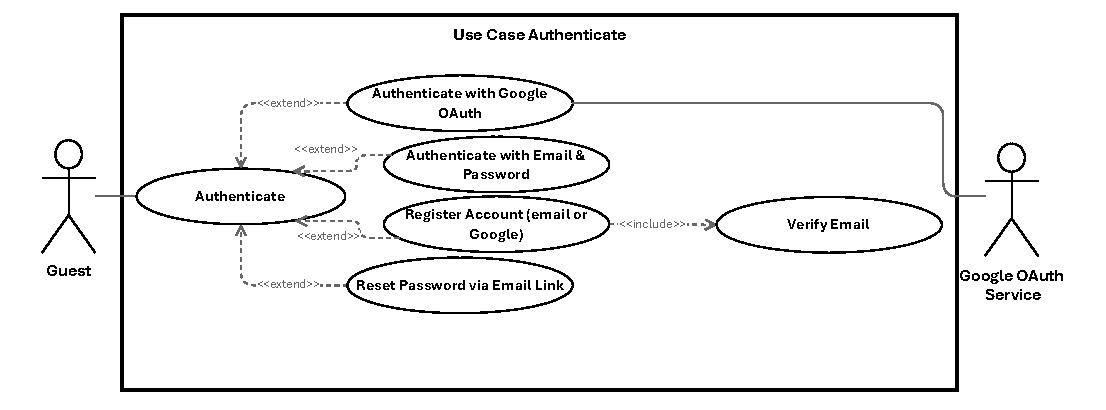
\includegraphics[width=\textwidth]{assets/chapter3/guest-authenticate-use-case}
    \caption{Use Case Authenticate}
    \label{fig:guest-authenticate-use-case}
\end{figure}
\dotsection{\textbf{Specification of the Use Case Authenticate with Google OAuth}}
\begin{table}[H]
    \centering
    \caption{Use Case Specification: Authenticate with Google OAuth}
    \begin{tabular}{|p{3.5cm}|p{10.5cm}|}
        \hline
        \textbf{Title}          & Authenticate with Google OAuth                                                                                                                     \\ \hline
        \textbf{Summary}        & Guest authenticates to the platform using a Google account through the OAuth 2.0 protocol, enabling single sign-on without manual credential entry \\ \hline
        \textbf{Primary Actor}  & Unauthenticated User (Guest)                                                                                                                       \\ \hline
        \textbf{Secondary Actor} & Google OAuth Service                                                                                                                                            \\ \hline
        \textbf{Precondition}   & The guest has a valid Google account; the Google OAuth integration is configured and active                                                        \\ \hline
        \textbf{Post-condition} & The guest is authenticated and redirected to the role-appropriate dashboard, or prompted to select a role if a new account                         \\ \hline
        \textbf{Basic Scenario} & \begin{minipage}[t]{\linewidth}
                                      \begin{enumerate}[topsep=0pt,itemsep=1pt,parsep=0pt,partopsep=0pt]
                                          \item Guest clicks the Google Sign-In button on the login or registration page
                                          \item System redirects the guest to the Google OAuth consent screen
                                          \item Guest authorizes the application and Google returns an authorization code
                                          \item System exchanges the authorization code for user profile information
                                          \item If the Google account matches an existing user, the system logs the user in
                                          \item If the Google account is new, the system creates a pending account and presents
                                                the role selection page
                                          \item Guest selects a role (Engineer or Teacher) and completes the signup
                                          \item System authenticates the user and redirects to the appropriate dashboard
                                      \end{enumerate}
                                  \end{minipage}                                                       \\ \hline
        \textbf{Error Scenario} & \begin{minipage}[t]{\linewidth}
                                      \begin{enumerate}[topsep=0pt,itemsep=1pt,parsep=0pt,partopsep=0pt]
                                          \item If the Google OAuth callback fails, the system redirects to the login page with
                                                an error message
                                          \item If the guest denies consent on the Google screen, the system returns to the
                                                login page
                                          \item If the Google account email is already linked to a password-based account, the
                                                system prompts the user to log in with email and password
                                      \end{enumerate}
                                  \end{minipage}                                                       \\ \hline
    \end{tabular}
    \label{tab:guest-google-oauth}
\end{table}
\dotsection{\textbf{Specification of the Use Case Authenticate with Email \& Password}}
\begin{table}[H]
    \centering
    \caption{Use Case Specification: Authenticate with Email \& Password}
    \begin{tabular}{|p{3.5cm}|p{10.5cm}|}
        \hline
        \textbf{Title}          & Authenticate with Email \& Password                                                          \\
        \hline
        \textbf{Summary}        & Guest authenticates to the platform using email and password to access protected features    \\
        \hline
        \textbf{Actor}          & Guest                                                                                        \\
        \hline
        \textbf{Precondition}   & The guest has a registered and verified account                                              \\
        \hline
        \textbf{Post-condition} & The guest is authenticated and receives a session with their assigned role                   \\
        \hline
        \textbf{Basic Scenario} & \begin{minipage}[t]{\linewidth}
                                      \begin{enumerate}[topsep=0pt,itemsep=1pt,parsep=0pt,partopsep=0pt]
                                          \item Guest navigates to the login page
                                          \item System displays the login form with email and password fields and a Google
                                                OAuth button
                                          \item Guest enters their credentials and submits the form
                                          \item System validates the credentials against the stored hash
                                          \item System creates an authenticated session with the user's role
                                          \item System redirects the guest to their role-specific dashboard
                                      \end{enumerate}
                                  \end{minipage}      \\
        \hline
        \textbf{Error Scenario} & \begin{minipage}[t]{\linewidth}
                                      \begin{enumerate}[topsep=0pt,itemsep=1pt,parsep=0pt,partopsep=0pt]
                                          \item If the credentials are invalid, the system displays an error and increments the
                                                failed attempt counter
                                          \item If the account is locked due to excessive failed attempts, the system prompts
                                                the guest to reset their password
                                          \item If Google OAuth fails, the system falls back to the email/password login form
                                      \end{enumerate}
                                  \end{minipage} \\
        \hline
    \end{tabular}
    \label{tab:guest-login}
\end{table}
\dotsection{\textbf{Specification of the Use Case Register Account (email or Google)}}
\begin{table}[H]
    \centering
    \caption{Use Case Specification: Register Account (email or Google)}
    \begin{tabular}{|p{3.5cm}|p{10.5cm}|}
        \hline
        \textbf{Title}          & Register Account (email or Google)                                                       \\
        \hline
        \textbf{Actor}          & Guest                                                                                    \\
        \hline
        \textbf{Precondition}   & The guest is not authenticated and the platform allows new registrations                 \\
        \hline
        \textbf{Post-condition} & A new user account is created with pending email verification status                     \\
        \hline
        \textbf{Basic Scenario} & \begin{minipage}[t]{\linewidth}
                                      \begin{enumerate}[topsep=0pt,itemsep=1pt,parsep=0pt,partopsep=0pt]
                                          \item Guest navigates to the registration page
                                          \item System displays the registration form with required fields
                                          \item Guest enters their name, email address, and password
                                          \item System validates the input fields and checks for duplicate email
                                          \item System creates the account with pending verification status
                                          \item System sends a verification email to the provided address
                                          \item Guest clicks the verification link to activate the account
                                      \end{enumerate}
                                  \end{minipage}            \\
        \hline
        \textbf{Error Scenario} & \begin{minipage}[t]{\linewidth}
                                      \begin{enumerate}[topsep=0pt,itemsep=1pt,parsep=0pt,partopsep=0pt]
                                          \item If the email is already registered, the system prompts the guest to log in
                                                instead
                                          \item If the password does not meet security requirements, the system rejects the
                                                submission
                                          \item If the verification email expires, the system allows resending a new link
                                      \end{enumerate}
                                  \end{minipage} \\
        \hline
    \end{tabular}
    \label{tab:guest-register}
\end{table}
\dotsection{\textbf{Specification of the Use Case Reset Password via Email Link}}
\begin{table}[H]
    \centering
    \caption{Use Case Specification: Reset Password via Email Link}
    \begin{tabular}{|p{3.5cm}|p{10.5cm}|}
        \hline
        \textbf{Title}          & Reset Password via Email Link                                                              \\ \hline
        \textbf{Summary}        & Guest, engineer, or teacher resets their password via email link                           \\
        \hline
        \textbf{Actor}          & Unauthenticated User (Guest), Engineer, Teacher                                            \\
        \hline
        \textbf{Precondition}   & The user has an active account with a registered email                                     \\
        \hline
        \textbf{Post-condition} & The user's password is updated and they can log in with the new password                   \\
        \hline
        \textbf{Basic Scenario} & \begin{minipage}[t]{\linewidth}
                                      \begin{enumerate}[topsep=0pt,itemsep=1pt,parsep=0pt,partopsep=0pt]
                                          \item User clicks "Forgot Password" on the login page
                                          \item User enters their email address
                                          \item System validates the email and creates a password reset token
                                          \item System sends a password reset email with a secure link
                                          \item User clicks the link and is redirected to the reset form
                                          \item User enters and confirms a new password
                                          \item System validates the password meets security requirements
                                          \item System updates the password and invalidates the reset token
                                          \item System notifies the user via email that the password was changed
                                      \end{enumerate}
                                  \end{minipage}              \\
        \hline
        \textbf{Error Scenario} & \begin{minipage}[t]{\linewidth}
                                      \begin{enumerate}[topsep=0pt,itemsep=1pt,parsep=0pt,partopsep=0pt]
                                          \item If the email is not registered, the system displays a generic success message
                                                (security)
                                          \item If the reset token expires, the system prompts the user to request a new one
                                          \item If the new password does not meet requirements, validation fails
                                      \end{enumerate}
                                  \end{minipage} \\
        \hline
    \end{tabular}
    \label{tab:guest-reset-pw}
\end{table}
\dotsection{\textbf{Specification of the Use Case Verify Email}}
\begin{table}[H]
    \centering
    \caption{Use Case Specification: Verify Email}
    \begin{tabular}{|p{3.5cm}|p{10.5cm}|}
        \hline
        \textbf{Title}          & Verify Email                                                                        \\ \hline
        \textbf{Summary}        & Guest, engineer, or teacher verifies their email address to activate their account  \\
        \hline
        \textbf{Actor}          & Unauthenticated User (Guest), Engineer, Teacher                                     \\
        \hline
        \textbf{Precondition}   & The user has registered an account but not verified their email                     \\
        \hline
        \textbf{Post-condition} & The user's email is marked as verified and full account access is granted           \\
        \hline
        \textbf{Basic Scenario} & \begin{minipage}[t]{\linewidth}
                                      \begin{enumerate}[topsep=0pt,itemsep=1pt,parsep=0pt,partopsep=0pt]
                                          \item User registers a new account or logs in with an unverified email
                                          \item System creates an email verification token
                                          \item System sends a verification email with a secure link
                                          \item User clicks the link and is redirected to the verification endpoint
                                          \item System validates the token and marks the email as verified
                                          \item System notifies the user that verification was successful
                                          \item User is redirected to their dashboard with full access
                                      \end{enumerate}
                                  \end{minipage}    \\
        \hline
        \textbf{Error Scenario} & \begin{minipage}[t]{\linewidth}
                                      \begin{enumerate}[topsep=0pt,itemsep=1pt,parsep=0pt,partopsep=0pt]
                                          \item If the token expires, the system prompts the user to request a new one
                                          \item If the token is invalid, the system displays an error message
                                          \item If the email is already verified, the system notifies the user
                                      \end{enumerate}
                                  \end{minipage} \\
        \hline
    \end{tabular}
    \label{tab:guest-verify-em}
\end{table}

\iffalse
\subsubsubsection[Consume Learning Content]{Refinement of the Use Case Consume Learning Content}
Figure \ref{fig:guest-consume-learning-content-use-case} presents the refinement of the Use Case Consume Learning Content for the Guest actor. This use case includes the following sub-use cases:
\begin{figure}[H]
    \centering
    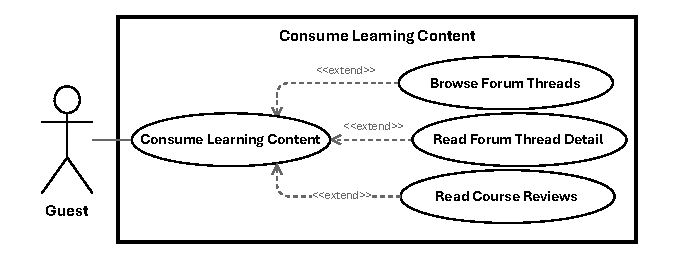
\includegraphics[width=\textwidth]{assets/chapter3/guest-consume-learning-content-use-case}
    \caption{Use Case Consume Learning Content}
    \label{fig:guest-consume-learning-content-use-case}
\end{figure}
\dotsection{\textbf{Specification of the Use Case Browse Forum Threads}}
\begin{table}[H]
    \centering
    \caption{Use Case Specification: Browse Forum Threads}
    \begin{tabular}{|p{3.5cm}|p{10.5cm}|}
        \hline
        \textbf{Title}          & Browse Forum Threads                                                                        \\
        \hline
        \textbf{Summary}        & Guest browses public forum threads to read community discussions without authentication     \\
        \hline
        \textbf{Actor}          & Guest                                                                                       \\
        \hline
        \textbf{Precondition}   & The platform is publicly accessible and the forum contains published threads                \\
        \hline
        \textbf{Post-condition} & The guest views forum thread listings and individual thread content                         \\
        \hline
        \textbf{Basic Scenario} & \begin{minipage}[t]{\linewidth}
                                      \begin{enumerate}[topsep=0pt,itemsep=1pt,parsep=0pt,partopsep=0pt]
                                          \item Guest navigates to the public forum page
                                          \item System displays a paginated list of public forum threads with titles, authors,
                                                and reply counts
                                          \item Guest selects a thread to read the original post and replies
                                          \item System displays the thread content and all approved replies
                                          \item Guest may sort threads by date, popularity, or category
                                          \item Guest may use the search function to find threads by keyword
                                      \end{enumerate}
                                  \end{minipage} \\
        \hline
        \textbf{Error Scenario} & \begin{minipage}[t]{\linewidth}
                                      \begin{enumerate}[topsep=0pt,itemsep=1pt,parsep=0pt,partopsep=0pt]
                                          \item If no threads match the search query, the system displays a no-results message
                                          \item If the thread has been deleted, the system shows a not-found notice
                                          \item If the guest attempts to post or reply, the system redirects to the
                                                registration page
                                      \end{enumerate}
                                  \end{minipage} \\
        \hline
    \end{tabular}
    \label{tab:guest-browse-forum}
\end{table}
\dotsection{\textbf{Specification of the Use Case Read Forum Thread Detail}}
\begin{table}[H]
    \centering
    \caption{Use Case Specification: Read Forum Thread Detail}
    \begin{tabular}{|p{3.5cm}|p{10.5cm}|}
        \hline
        \textbf{Title}          & Read Forum Thread Detail                                                                    \\ \hline
        \textbf{Summary}        & Guest reads the full content of a specific forum thread including original post and replies \\ \hline
        \textbf{Actor}          & Unauthenticated User (Guest)                                                                \\ \hline
        \textbf{Precondition}   & The forum thread is published and publicly accessible                                       \\ \hline
        \textbf{Post-condition} & The guest views the complete thread content with all approved replies                       \\ \hline
        \textbf{Basic Scenario} & \begin{minipage}[t]{\linewidth}
                                      \begin{enumerate}[topsep=0pt,itemsep=1pt,parsep=0pt,partopsep=0pt]
                                          \item Guest selects a forum thread from the thread listing
                                          \item System displays the thread detail page
                                          \item System shows the original post with author, timestamp, and content
                                          \item System displays all approved replies in chronological order
                                          \item Guest may read the full discussion thread
                                          \item Guest may view reply counts and engagement metrics
                                      \end{enumerate}
                                  \end{minipage}             \\ \hline
        \textbf{Error Scenario} & \begin{minipage}[t]{\linewidth}
                                      \begin{enumerate}[topsep=0pt,itemsep=1pt,parsep=0pt,partopsep=0pt]
                                          \item If the thread is not found, the system displays a not-found message
                                          \item If the thread is unpublished, the system redirects to the forum listing
                                          \item If the guest attempts to post or reply, the system redirects to registration
                                      \end{enumerate}
                                  \end{minipage}   \\ \hline
    \end{tabular}
    \label{tab:guest-read-thread}
\end{table}
\dotsection{\textbf{Specification of the Use Case Read Course Reviews}}
\begin{table}[H]
    \centering
    \caption{Use Case Specification: Read Course Reviews}
    \begin{tabular}{|p{3.5cm}|p{10.5cm}|}
        \hline
        \textbf{Title}          & Read Course Reviews                                                              \\ \hline
        \textbf{Summary}        & Guest browses course reviews to evaluate training path quality                   \\
        \hline
        \textbf{Actor}          & Unauthenticated User (Guest), Engineer, Teacher, Administrator                   \\
        \hline
        \textbf{Precondition}   & The training path has approved reviews and is publicly visible                   \\
        \hline
        \textbf{Post-condition} & The guest views a list of course reviews with ratings and metadata               \\
        \hline
        \textbf{Basic Scenario} & \begin{minipage}[t]{\linewidth}
                                      \begin{enumerate}[topsep=0pt,itemsep=1pt,parsep=0pt,partopsep=0pt]
                                          \item Guest opens a training path detail page
                                          \item System displays the training path metadata including average rating
                                          \item Guest navigates to the Reviews tab
                                          \item System retrieves and displays approved reviews with pagination
                                          \item Guest filters reviews by rating, recency, or helpfulness
                                          \item Guest reads individual reviews
                                      \end{enumerate}
                                  \end{minipage} \\
        \hline
        \textbf{Error Scenario} & \begin{minipage}[t]{\linewidth}
                                      \begin{enumerate}[topsep=0pt,itemsep=1pt,parsep=0pt,partopsep=0pt]
                                          \item If no reviews exist, the system displays an empty-state message
                                          \item If the training path is not approved, reviews are not shown
                                      \end{enumerate}
                                  \end{minipage}     \\
        \hline
    \end{tabular}
    \label{tab:guest-reviews}
\end{table}
\fi

\subsubsubsection[Verify a certificate]{Refinement of the Use Case Verify a certificate}
Figure \ref{fig:guest-consume-learning-content-use-case} presents the refinement of the Use Case Verify a certificate for the Guest actor. This use case includes the following sub-use cases:
\begin{figure}[H]
    \centering
    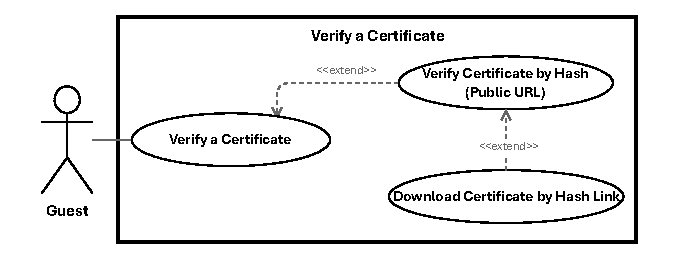
\includegraphics[width=\textwidth]{assets/chapter3/guest-verify-a-certificate-use-case}
    \caption{Use Case Verify a certificate}
    \label{fig:guest-verify-a-certificate-use-case}
\end{figure}

\dotsection{\textbf{Specification of the Use Case Verify a Certificate}}
\begin{table}[H]
    \centering
    \caption{Use Case Specification: Verify Certificate}
    \begin{tabular}{|p{3.5cm}|p{10.5cm}|}
        \hline
        \textbf{Title}          & Verify Certificate                                                                     \\ \hline
        \textbf{Summary}        & Guest verifies the authenticity of a digital certificate using its hash                \\
        \hline
        \textbf{Actor}          & Unauthenticated User (Guest)                                                           \\
        \hline
        \textbf{Precondition}   & The certificate exists and has been issued by the platform                             \\
        \hline
        \textbf{Post-condition} & The guest receives confirmation of the certificate's validity and details              \\
        \hline
        \textbf{Basic Scenario} & \begin{minipage}[t]{\linewidth}
                                      \begin{enumerate}[topsep=0pt,itemsep=1pt,parsep=0pt,partopsep=0pt]
                                          \item Guest receives a certificate (e.g., via email or LinkedIn)
                                          \item Guest navigates to the certificate verification page
                                          \item Guest enters the certificate hash (or clicks a verification link)
                                          \item System validates the hash and retrieves the certificate record
                                          \item System displays the certificate details: recipient name, issue date, and
                                                credential title
                                          \item System confirms the certificate is authentic and not revoked
                                      \end{enumerate}
                                  \end{minipage}  \\
        \hline
        \textbf{Error Scenario} & \begin{minipage}[t]{\linewidth}
                                      \begin{enumerate}[topsep=0pt,itemsep=1pt,parsep=0pt,partopsep=0pt]
                                          \item If the hash is invalid, the system displays an error message
                                          \item If the certificate is revoked, the system notifies the guest
                                          \item If the certificate has expired, the system displays an expiration warning
                                      \end{enumerate}
                                  \end{minipage} \\
        \hline
    \end{tabular}
    \label{tab:guest-verify-cert}
\end{table}
\dotsection{\textbf{Download Certificate by Hash Link}}
\begin{table}[H]
    \centering
    \caption{Use Case Specification: Download Certificate by Hash Link}
    \begin{tabular}{|p{3.5cm}|p{10.5cm}|}
        \hline
        \textbf{Title}          & Download Certificate by Hash Link                                                           \\ \hline
        \textbf{Summary}        & Guest downloads a digital certificate using a verification hash link without authentication \\ \hline
        \textbf{Actor}          & Unauthenticated User (Guest)                                                                \\ \hline
        \textbf{Precondition}   & The certificate exists, is valid, and has not been revoked                                  \\ \hline
        \textbf{Post-condition} & The guest downloads the certificate file in PDF or image format                             \\ \hline
        \textbf{Basic Scenario} & \begin{minipage}[t]{\linewidth}
                                      \begin{enumerate}[topsep=0pt,itemsep=1pt,parsep=0pt,partopsep=0pt]
                                          \item Guest receives a certificate download link via email or external platform
                                          \item Guest clicks the download link containing the certificate hash
                                          \item System validates the hash and retrieves the certificate record
                                          \item System confirms the certificate is valid and not revoked
                                          \item System generates and serves the certificate file for download
                                          \item Guest saves the certificate file to their device
                                      \end{enumerate}
                                  \end{minipage}      \\ \hline
        \textbf{Error Scenario} & \begin{minipage}[t]{\linewidth}
                                      \begin{enumerate}[topsep=0pt,itemsep=1pt,parsep=0pt,partopsep=0pt]
                                          \item If the hash is invalid, the system displays an error message
                                          \item If the certificate is revoked, the system notifies the guest
                                          \item If the certificate has expired, the system displays an expiration warning
                                          \item If the download fails, the system offers a retry option
                                      \end{enumerate}
                                  \end{minipage}      \\ \hline
    \end{tabular}
    \label{tab:guest-download-cert}
\end{table}

